%!TEX root = ../dissertation.tex


\chapter{What do you do if you hhave a really really long chapter name? well sometimes it breaks up the line and sometimes it doesn't so you have to use something called chaptermark...} \label{chap:dataset}
\chaptermark{You see, shorter title}

\textbf{Abstract:} \hspace{0.5cm}
\textit{
If your thesis is in need for english chapter abstract
}
\\

\noindent \textbf{Résumé:} \hspace{0.5cm}
\textit{
If your thesis is in need for french chapter abstract}


\newpage
\minitoc
\newpage

\section{Adding figures and horizontal captions}
Here I show an example where I use subfloat to position the images like on a grid but also adding horizontal caption.


\begin{figure}[!t]
    \centering
    \subfloat{\raisebox{1.5cm}{\makebox[0pt]{\rotatebox[origin=c]{90}{
  {\footnotesize (a) Release 1.}}
    }\hspace*{2em}}\hspace{-0.5cm}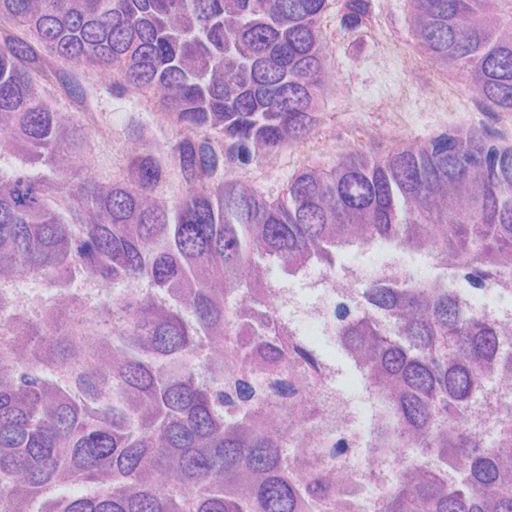
\includegraphics[width=\tilesize]{release1/RGB_04_1}
    \label{release1:rgb1}}
    \hfil
    \subfloat{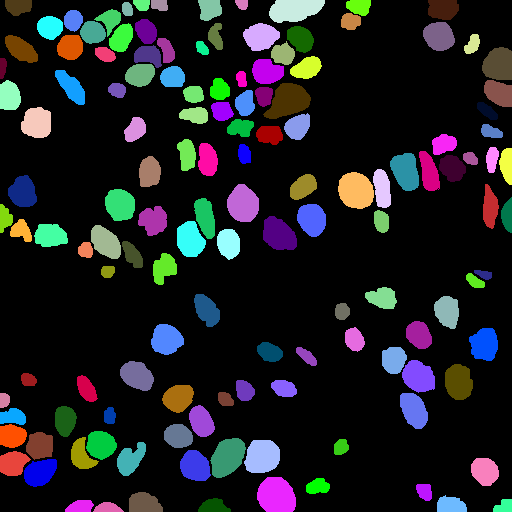
\includegraphics[width=\tilesize]{release1/GT_04_1}
    \label{release1:gt1}}
    \hfil
    \subfloat{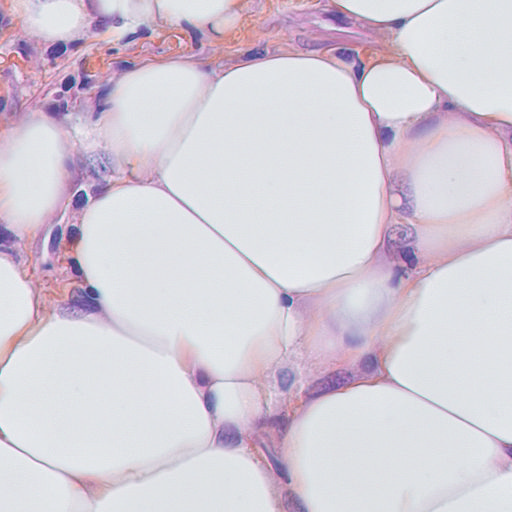
\includegraphics[width=\tilesize]{release1/RGB_04_7}
    \label{release1:rgb2}}
    \hfil
    \subfloat{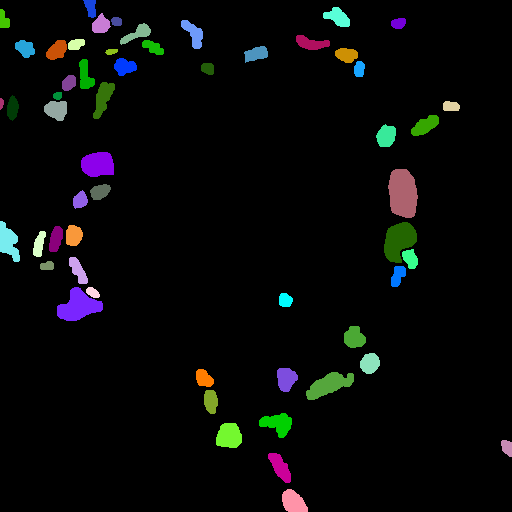
\includegraphics[width=\tilesize]{release1/GT_04_7}
    \label{release1:gt2}}

    \centering
    \subfloat{\raisebox{1.5cm}{\makebox[0pt]{\rotatebox[origin=c]{90}{
  {\footnotesize (b) Release 2.}}
    }\hspace*{2em}}\hspace{-0.5cm}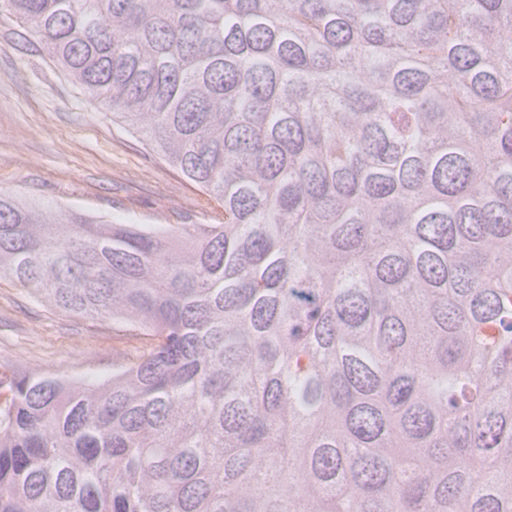
\includegraphics[width=\tilesize]{release2/Slide_1_1}
    \label{release2:rgb1}}
    \hfil
    \subfloat{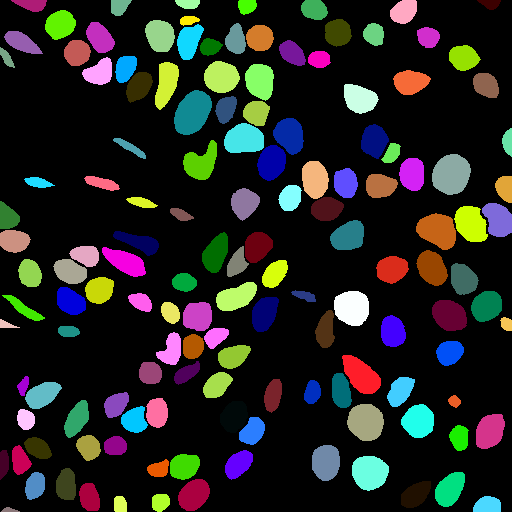
\includegraphics[width=\tilesize]{release2/GT_1_1}
    \label{release2:gt1}}
    \subfloat{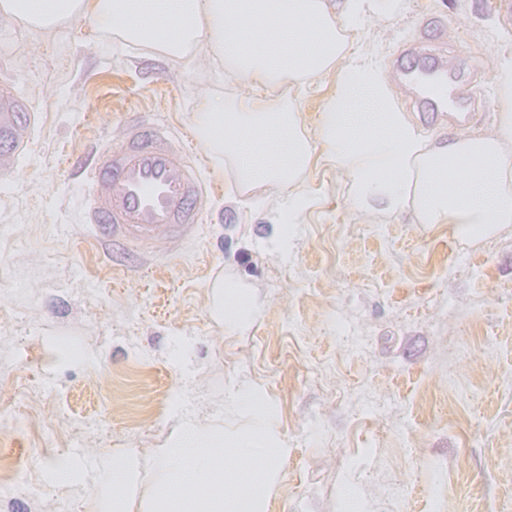
\includegraphics[width=\tilesize]{release2/Slide_1_2}
    \label{release2:rgb2}}
    \hfil
    \subfloat{
\includegraphics[width=\tilesize]{release2/GT_1_2}
    \label{release2:gt2}}
    \setcounter{subfigure}{3} %useful to change 

    \centering
    \subfloat[Raw data.]{\raisebox{1.5cm}{\makebox[0pt]{\rotatebox[origin=c]{90}{
  {\footnotesize (c) Release 4.}}
    }\hspace*{2em}}\hspace{-0.5cm}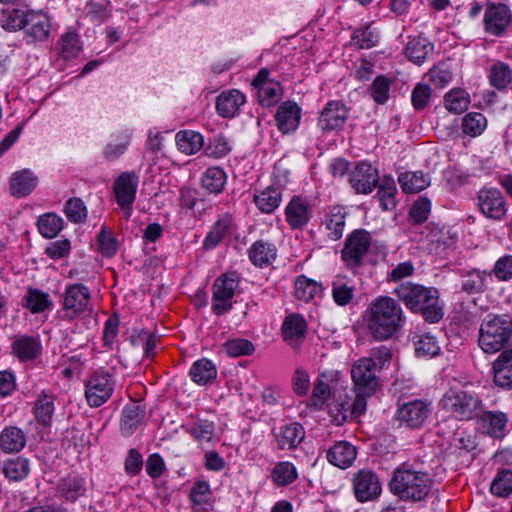
\includegraphics[width=\tilesize]{release3/RGB_13_6}
    \label{release3:rgb1}}
    \hfil
    \subfloat[Ground Truth.]{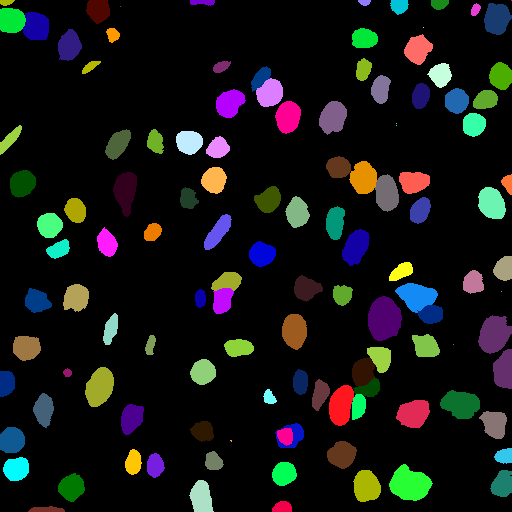
\includegraphics[width=\tilesize]{release3/GT_13_6}
    \label{release3:gt1}}
    \subfloat[Raw data.]{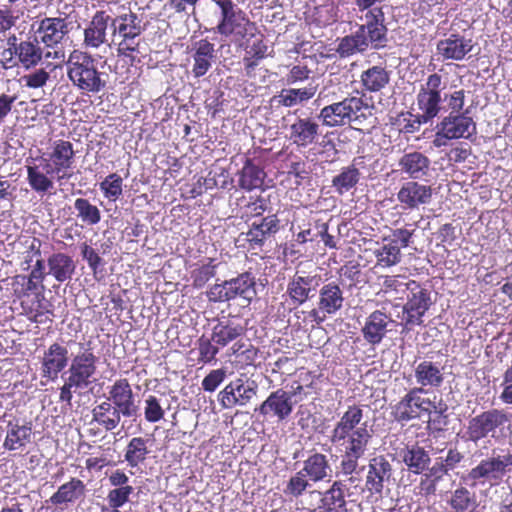
\includegraphics[width=\tilesize]{release3/RGB_14_2}
    \label{release3:rgb2}}
    \hfil
    \subfloat[Ground truth.]{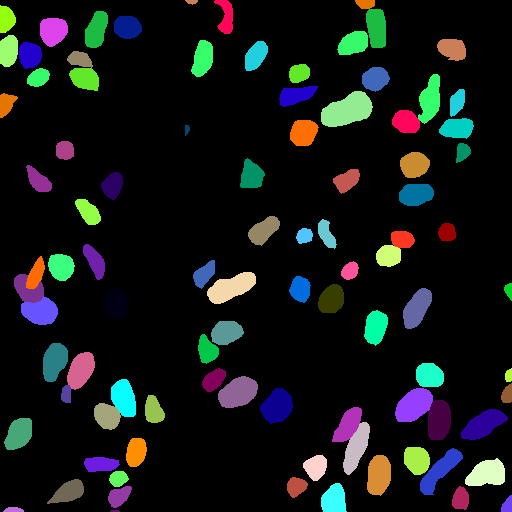
\includegraphics[width=\tilesize]{release3/GT_14_2}
    \label{dataset1:release3:gt2}}
    \caption{Just doing some publicity, but this is my dataset if you want to use it for segmentation or machine learning purposes... :D The database: \cite{database_nuclei_seg}, the associated paper: \cite{naylor2018segmentation}.}
    \label{my_dataset}
\end{figure}

\section{Shrinking large tables}

\begin{table}
    \begin{center}
        \resizebox{0.9\linewidth}{!}{%<----
            \begin{tabular}{l|rrrrrrrrrrrrrr|r}
            \hline
            Slide number &  01 &  02 &  03 &  04 &  05 &  06 &  07 &  08 &  09 &  10 &  11 &  12 &  13 &  14 &  Total \\
            \hline
            Number of patches & 7 & 3 & 5 & 8 & 4 & 3 & 3 & 4 & 6 & 4 & 3 & 7 & 6 & 5 & 68 \\
            \hline
            \hline
            Adipocyte &        0 &        1 &        0 &       32 &        0 &        0 &        0 &        0 &        5 &        1 &        0 &        0 &        0 &        0 &     39 \\
            Cancerous &      243 &      150 &      133 &      443 &      306 &      110 &       48 &      187 &      178 &      192 &      141 &      230 &      274 &      326 &   2961 \\
            Endothelial &      12 &        0 &        0 &        7 &        0 &        3 &        6 &       35 &        3 &        7 &        8 &        5 &       11 &        6 &    103 \\
            Epithelial &      22 &        0 &        0 &        0 &        0 &        0 &       34 &        0 &        0 &        0 &        0 &        0 &        0 &        0 &     56 \\
            Fibroblast &      136 &        8 &       95 &       92 &      105 &       85 &      155 &        5 &        1 &        9 &       97 &        0 &        0 &        0 &    788 \\
            Glial     &        0 &        0 &        0 &        0 &        0 &        0 &        0 &        0 &        0 &        0 &        0 &       63 &       46 &       50 &    159 \\
        Lympho/Plasmocyte&       43 &       29 &       58 &       20 &        8 &        6 &      307 &      212 &      103 &      105 &        6 &        0 &        2 &        0 &    899 \\
            Mitosis    &        2 &        0 &        1 &        2 &        0 &        0 &        0 &        6 &       11 &        2 &        2 &        0 &        1 &        0 &     27 \\
            Myoepithelial  &  0 &        0 &        0 &        0 &        0 &        0 &        4 &        0 &        0 &        0 &        0 &        0 &        0 &        0 &      4 \\
            Necrosis   &        0 &        0 &        0 &        0 &        0 &        0 &        1 &        0 &        0 &        0 &        0 &        0 &        0 &        0 &      1 \\
            Neurons &        0 &        0 &        0 &        0 &        0 &        0 &        0 &        0 &        0 &        0 &        0 &        0 &        9 &        0 &      9 \\
            Unknown   &        0 &        0 &        0 &        0 &        0 &        0 &        0 &        0 &        0 &        0 &        0 &        9 &        3 &       92 &    104 \\
            \hline
            Total     &      458 &      188 &      287 &      596 &      419 &      204 &      555 &      445 &      301 &      316 &      254 &      307 &      346 &      474 &   5150 \\
            \hline
            \end{tabular}%
}
    \end{center}
    \caption{Example of a large table that whose size is adjusted with resizebox, this is the 3rd release if you were wondering how we jumped from 2 to 4 in the previous captions... \ref{release1:rgb1} and \ref{release1:gt1}}
    \label{table:full_type_table}
\end{table}


Some of the data was downloaded from the TCGA website \cite{TCGAwebsite}.
